%!TEX program = xelatex
\documentclass{beamer}

\usepackage{blindtext}
\usepackage[absolute,overlay]{textpos}
\usepackage{graphicx} % for pdf, bitmapped graphics files
\graphicspath{ {gm22may2018/images/} }

\usetheme{Execushares}
\def\checkmark{\tikz\fill[scale=0.4](0,.35) -- (.25,0) -- (1,.7) -- (.25,.15) -- cycle;}

\title{Back-Pressure based NoC to provide guaranteed and In-Order packet deliveries}
\subtitle{An overall review of how things stand right now}
\author{Gurshaant Malik}
\date{\today}

\setcounter{showSlideNumbers}{1}

\begin{document}
	\frame{\titlepage}
	\begin{frame}
		\frametitle{What are the 4 designs?}
		\pause
		\begin{enumerate}
			\item The back-pressure based design.
			\pause
			\item The local deflection based design.
			\pause 
			\item CMU CONNECT.
			\pause
			\item AXI-4 Stream Interconnect.\pause(A Xilinx IP).
		\end{enumerate}
	\end{frame}

	\setcounter{showProgressBar}{1}
	\setcounter{showSlideNumbers}{1}
	
	\section{CMU Connect}
	
	    \begin{frame}\frametitle{Specifications}
	    \begin{textblock*}{3.5cm}(3.5cm, 2.5cm) % {block width} (coords)
	        \visible<1>{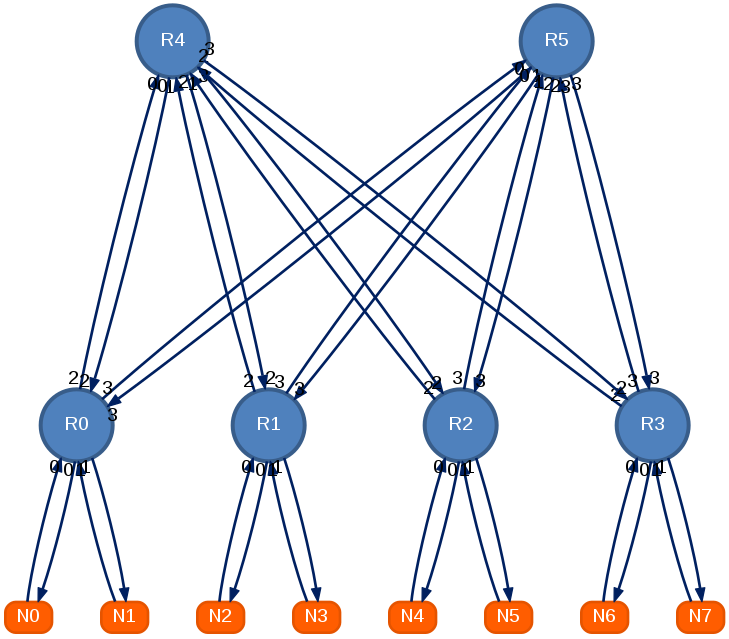
\includegraphics[scale=0.25]{cmu_connect.png}}
	    \end{textblock*}
	    \pause
	    \begin{itemize}
	        \item Simple Input Queued.
	        \pause
	        \begin{itemize}
	            \item Flit buffer depth = 8.
	        \end{itemize}
	        \pause
	        \item Peak Flow Control
	        \pause
	        \begin{itemize}
	            \item No Virtual Links.
	        \end{itemize}
	        \pause
	        \item Separate Input-First Round-Robin allocator.
	    \end{itemize}
	    \pause
	    \begin{textblock*}{3cm}(9cm, 5.5cm) % {block width} (coords)
            \visible<2,3,4,5,6>{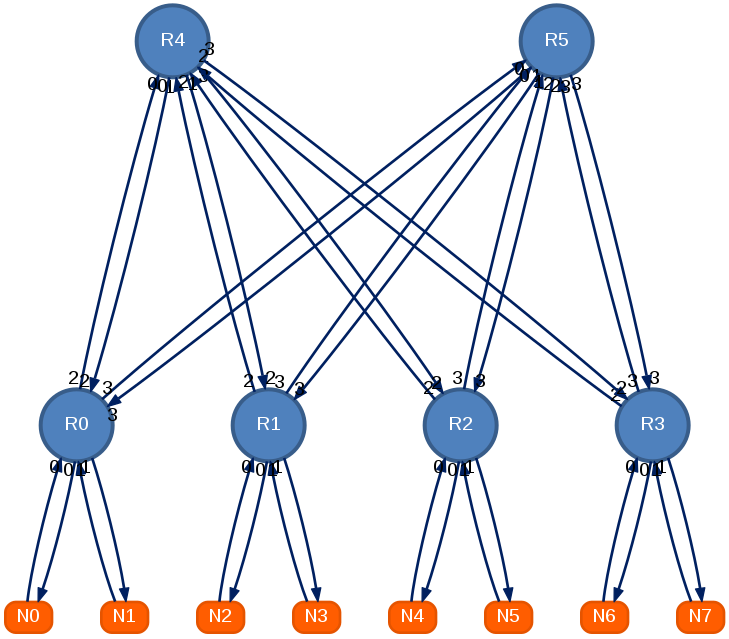
\includegraphics[height=3.5cm, width=3.5cm]{cmu_connect.png}}
        \end{textblock*}
	    \end{frame}
	    
	    \begin{frame}\frametitle{Advantages}
	    \pause
	    \begin{itemize}
	        \item Provide In-Order delivery.
	        \pause
	        \item Guaranteed packet delivery.
	        \pause
	        \item High throughput.
        \end{itemize}
	    \end{frame}
	    
	    \begin{frame}\frametitle{Disadvantages}
	    \pause
	    \begin{itemize}
	        \item Bloated design. High area consumption.
	        \pause
	        \item Slow peak frequency.
	        \pause
	        \item Not scalable. Supports maximum of 64 clients.
        \end{itemize}
	    \end{frame}
	
	\section{The Back-Pressure NoC}
        \begin{frame}
        \frametitle{What are the design wins?}
           \pause
           It is the only design that achieves all of the following:
           \pause
           \begin{itemize}
               \item Guaranteed packet delivery.
               \pause 
               \item In-Order packet delivery.
               \pause
               \item Scales to support any number of clients.
               \pause
               \item FPGA resource efficient.
               \pause
               \item Meets frequency targets of 300MHz+
           \end{itemize}
        \end{frame}
        
        \begin{frame}{Checklist}
            \begin{center}
                \begin{tabular}{c c c c c} 
                    \hline
                    & \textbf{CMU} & \textbf{LD} & \textbf{AXI-IC} & \textbf{BP} \\ [0.5ex] 
                    \hline\hline
                    \pause
                    \textbf{Guaranteed Delivery} & \checkmark & X & \checkmark & \checkmark \\ 
                    \hline
                    \pause
                    \textbf{In-Order Delivery} & \checkmark & X & \checkmark & \checkmark \\ 
                    \hline
                    \pause
                    \textbf{Scalable} & X & \checkmark & X & \checkmark \\ 
                    \hline
                    \pause
                    \textbf{Frequency Targets} & X & \checkmark & \checkmark & \checkmark \\  
                    \hline
                \end{tabular}
            \end{center}
        \end{frame}
        
        \begin{frame}{Specifications:}
        \pause
            \begin{itemize}
                \item Round Robin. Ensures packet progress.
                \begin{itemize}
                    \pause
                    \item Fair.
                    \pause
                    \item Smart.
                \end{itemize}
                \pause
                \item Quantified up-stream paths. Ensures In-Order.
                \pause
                \begin{itemize}
                    \item Concrete path for each src-dest pair.
                \end{itemize}
                \pause
                \item Back-Pressure. Ensures In-Order.
                \pause
                \begin{itemize}
                    \item Younger flit cannot overtake older flit.
                \end{itemize}
            \end{itemize}
        \end{frame}



\end{document}
